<<<<<<< HEAD
\label{DefLevures}
=======
>>>>>>> 59e5d45cfb64c9e07b007057e56d42745e3a510b
\section{Les levures}
Les levures est des champignons unicellulaires aptes à provoquer la fermentation des matières organiques animales ou végétales. Les levures sont employées pour la fabrication du vin, de la bière, des alcools industriels, des pâtes levées et d'antibiotiques. Les levures sont des micro-organismes eucaryotes, ainsi possèdent-elles les caractéristiques structurelles propres à ce type cellulaire et d'autres plus spécifiques aux levures elles-mêmes. Il existe de nombreuse forme de levures qui ont des caractéristiques différentes. Par exemples les « levures de boulanger » (Saccharomyces cerevisiae) ont un processus de division complexe et assez différent des autres cellules : Elles forment des bourgeonnements. D’autres types de levures comme par exemples celles de souche Ade2 (souvent utilisés dans des expériences notamment  en génétique) se divisent normalement. De plus les levures possèdent deux principaux métabolismes :

\begin{itemize}
	\item La respiration classique en aérobie qui transforme glucose et oxygène en énergie, eau et CO2 
		\chimiecite{C_6H_{12}O_6 + 6O_2 \longrightarrow 6CO_2 + 6H_2 O + energie}
	\item La fermentation alcoolique qui permet de faire de l’énergie sans oxygène en produisant de l’éthanol  et du CO2

		\chimiecite{C_6H_{12}O_6 \longrightarrow 2CO_2 + 2CH_3CH_2OH  + energie}
\end{itemize}

\section{L’expérience souche Ade2 et UV}
\begin{figure}[H]
	\centering
	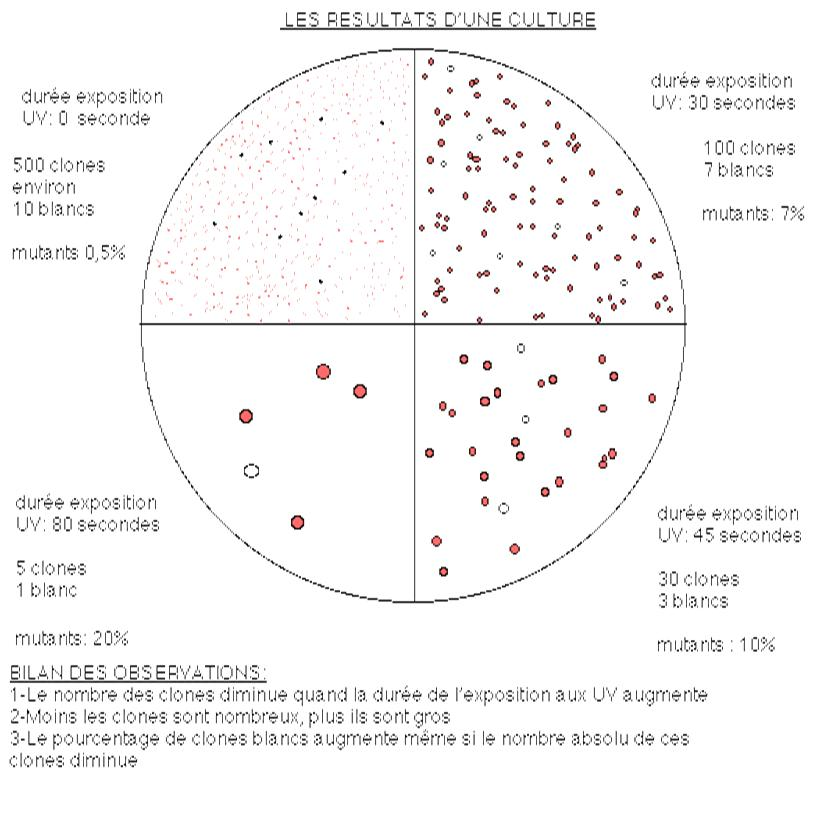
\includegraphics[width=26em]{Annexes/Images/lev.jpg}
	\caption{Résultats de l'expérience}
\end{figure}

Cette expérience montre deux effets des UV sur les cellules de levures :

Les mutations létales engendrées par les ultra-violets modifient les gènes essentiels au fonctionnement général de la cellule et finissent par la tuer. Ensuite certaines de ces levures qui ont résisté aux rayons ont mutées et cette même mutation engendre une modification de la couleur de ces individus. Grâce à cette expérience on peut déterminer le taux de mutation et de mort chez ces levures en cas d’exposition à l’UV…

Les observations de cette expérience concernant les mutations sont consignées dans ce tableau : 

\begin{center}
	\begin{tabular}{ c | c | c  }
	   Durée d’exposition aux UV (secondes) & Nombre de clones par cm² & Nombre total de clones blancs \\ \hline \hline
	   0 & 200 & 20 \\ \hline
	   30 & 22 & 3 \\ \hline
	   45 & 12 & 2 \\ \hline
	   80 & 7 & 1
	\end{tabular}
\end{center}


Ces informations on été tirées de Wikipédia, article sur les levures/Mutagenèse chez une souche de levure rose ADE 2 et sur le site \url{http://www.snv.jussieu.fr/vie/informations/2/22ADN/mutagenese/levureADE/levureade.htm} comme spécifié dans la sitographie, annexe \ref{BibSito}.

